\documentclass[a4paper,12pt]{article}

\usepackage{tma}
\usepackage{hyperref}
\usepackage{graphicx}
\usepackage{epstopdf} %%package to overcome problem with eps in pdf files


\graphicspath{{./image/}}


\myname{Anshul Mittal}
\mypin{13113017}
\mycourse{CSN-212: Assignment3}
% \mytma{01}

%\marginnotes

\begin{document}
\rule[0.4pt-1em]{0.4pt}{1em}\hrulefill\rule[0.4pt-1em]{0.4pt}{1em}
\begin{center}
\textbf{Code: Bellman Flyod}--\href{https://github.com/anshumitts/CSN212/tree/master/Ass3}{Click here}\newline
Link contains: 
\begin{itemize}
	\item main code file (bellford.cpp).
	\item Output file for large inputs(output.txt).
	\item raninput.py to make sample input.
\end{itemize}
\begin{figure}[!h]
  	\begin{minipage}{\linewidth}  
  	\begin{center}
    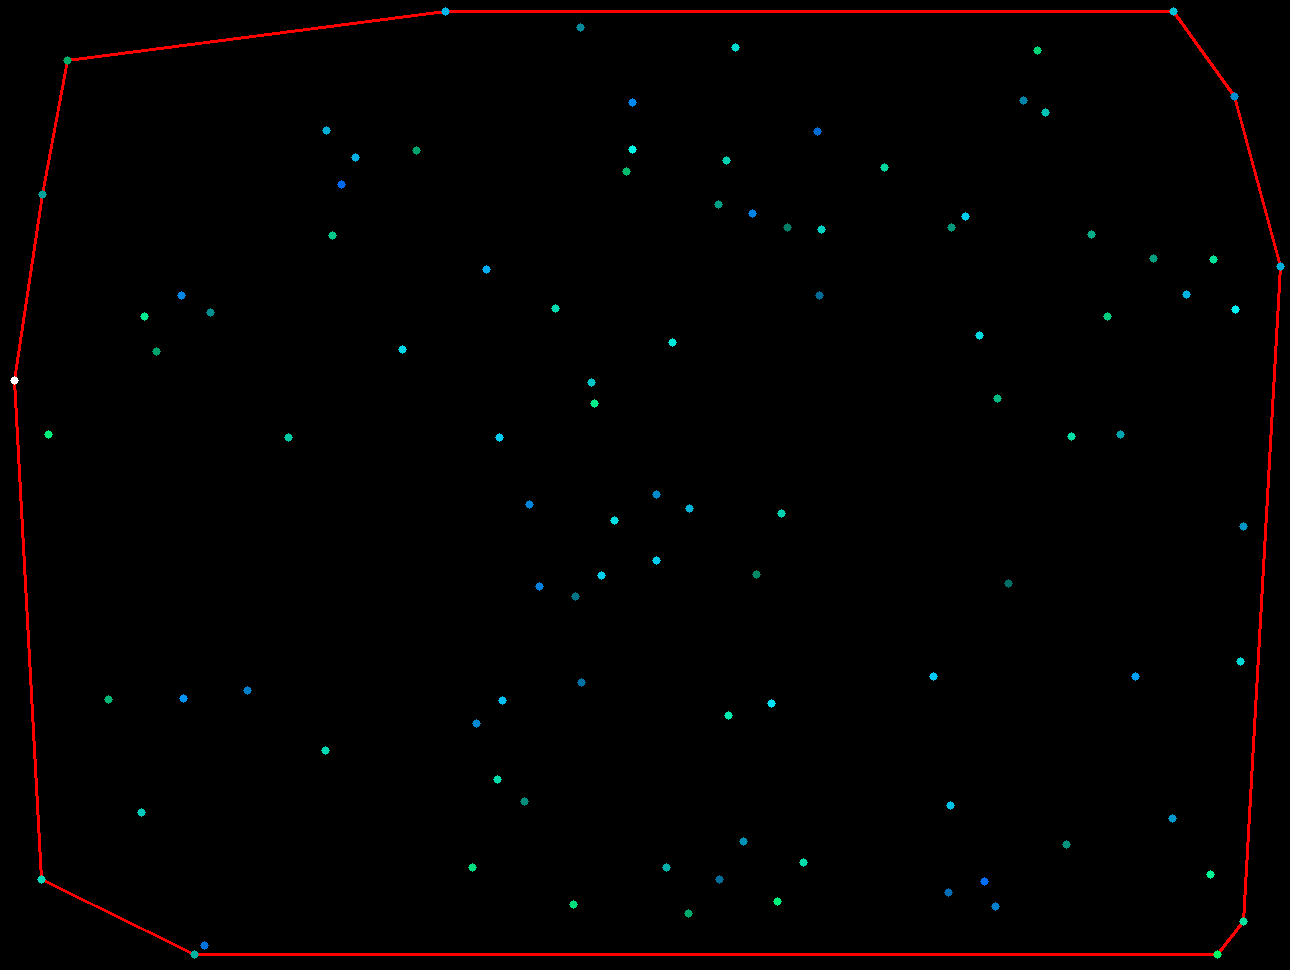
\includegraphics[width=0.72\textwidth]{/home/anshul/Documents/lastOne/DAA/CSN212/Ass3/files/1}
    \caption{Plot of Time, Vertex and Edges.}
    \end{center}
    \end{minipage}
	\begin{minipage}{\linewidth}  
	\begin{center}
    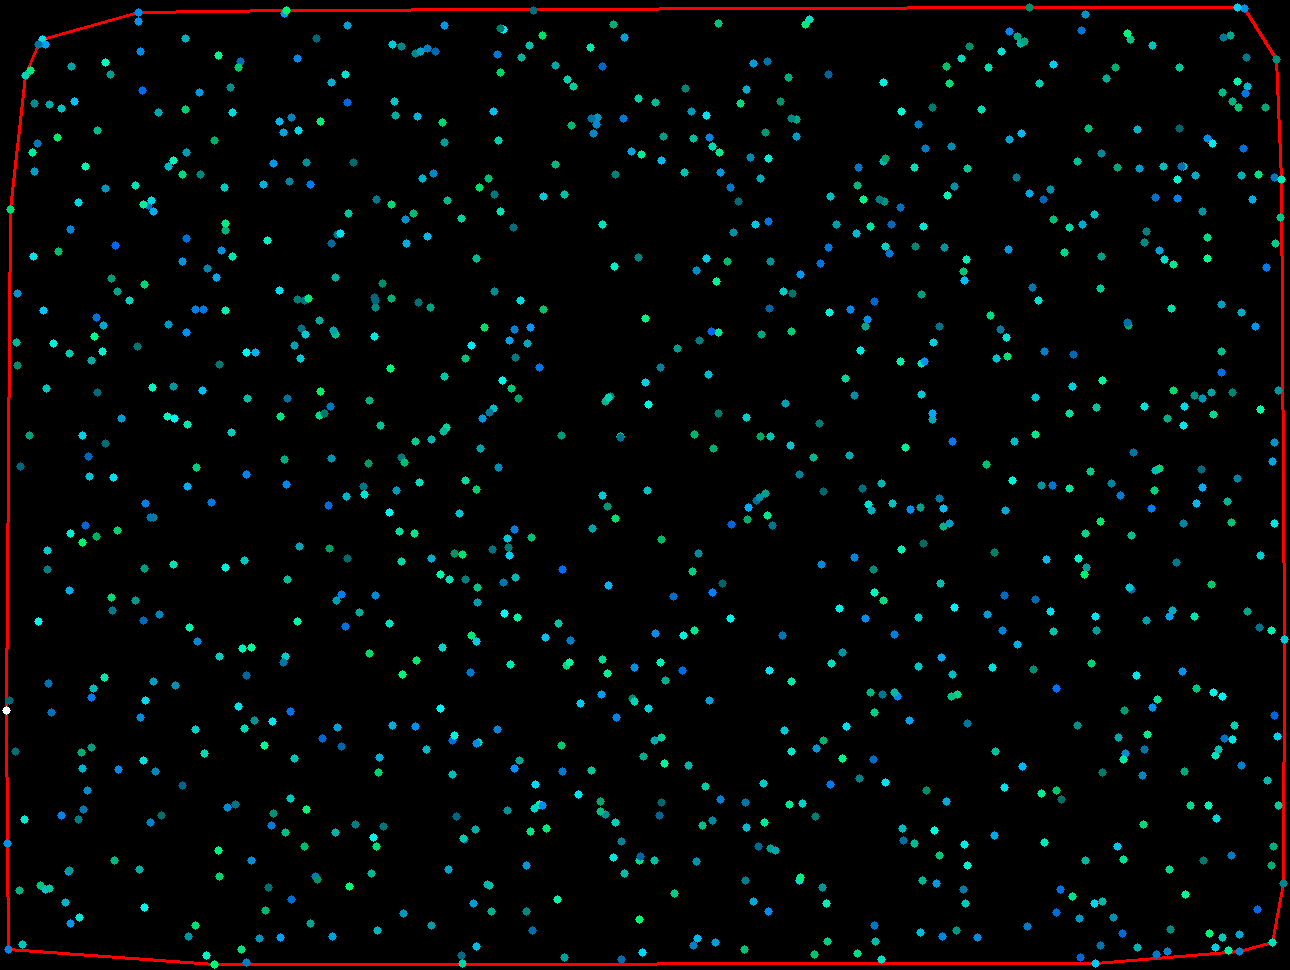
\includegraphics[width=0.72\textwidth]{/home/anshul/Documents/lastOne/DAA/CSN212/Ass3/files/2}
    \caption{Plot of Time and VxE(vertex V and Edges E).}
    \end{center}
    \end{minipage}
\end{figure}
\end{center}
\rule{0.4pt}{1em}\hrulefill\rule{0.4pt}{1em}
\end{document}

